%%%%%%%%%%%%%%%%%%%%%%%%%%%%%%%%%%%%%%%%%
% Short Sectioned Assignment
% LaTeX Template
% Version 1.0 (5/5/12)
%
% This template has been downloaded from:
% http://www.LaTeXTemplates.com
%
% Original author:
% Frits Wenneker (http://www.howtotex.com)
%
% License:
% CC BY-NC-SA 3.0 (http://creativecommons.org/licenses/by-nc-sa/3.0/)
%
%%%%%%%%%%%%%%%%%%%%%%%%%%%%%%%%%%%%%%%%%

%----------------------------------------------------------------------------------------
%	PACKAGES AND OTHER DOCUMENT CONFIGURATIONS
%----------------------------------------------------------------------------------------

\documentclass[paper=a4, fontsize=12pt]{scrartcl} % A4 paper and 11pt font size

\usepackage[T1]{fontenc} % Use 8-bit encoding that has 256 glyphs
\usepackage{fourier} % Use the Adobe Utopia font for the document
\usepackage[english]{babel} % English language/hyphenation
\usepackage{amsmath,amsfonts,amsthm} % Math packages
\usepackage{listings}
\lstset{basicstyle=\small\ttfamily, breaklines=truem, numbers=left, stepnumber=1,
        firstnumber=1, numberfirstline=true, keywordstyle=\bfseries\color{green!40!black},
        commentstyle=\itshape\color{purple!40!black}, identifierstyle=\color{blue},
        stringstyle=\color{orange}}

\usepackage{lipsum} % Used for inserting dummy 'Lorem ipsum' text into the template
\usepackage{tikz}
\usepackage[]{graphicx}

\usepackage{sectsty} % Allows customizing section commands
\allsectionsfont{\centering \normalfont\scshape}

\usepackage{fancyhdr} % Custom headers and footers
\pagestyle{fancyplain} % Makes all pages in the document conform to the custom headers and footers
\fancyhead{} % No page header - if you want one, create it in the same way as the footers below
\fancyfoot[L]{} % Empty left footer
\fancyfoot[C]{} % Empty center footer
\fancyfoot[R]{\thepage} % Page numbering for right footer
\renewcommand{\headrulewidth}{0pt} % Remove header underlines
\renewcommand{\footrulewidth}{0pt} % Remove footer underlines
\setlength{\headheight}{13.6pt} % Customize the height of the header

\numberwithin{equation}{section}
\numberwithin{figure}{section}
\numberwithin{table}{section}

\setlength\parindent{0pt}

\linespread{1.5}
%----------------------------------------------------------------------------------------
%	TITLE SECTION
%----------------------------------------------------------------------------------------

\newcommand{\horrule}[1]{\rule{\linewidth}{#1}} % Create horizontal rule command with height

\title{
\normalfont \normalsize
\textsc{EURECOM, Computation Methods for Digital Communication Systems} \\ [25pt]
\horrule{0.5pt} \\[0.4cm] % Thin top horizontal rule
\huge SSE/AVX SIMD Benchmarking \\ % The assignment title
\horrule{2pt} \\[0.5cm] % Thick bottom horizontal rule
}

\author{Simone Rossi} % Your name

\date{\normalsize\today} % Today's date or a custom date

\begin{document}

\maketitle % Print the title

%----------------------------------------------------------------------------------------
%	PROBLEM 1
%----------------------------------------------------------------------------------------

\section{Introduction}

In this laboratory, we studied the speedup that Single Instructions Multiple Data (SIMD)
instructions (mostly Intel SSE4 and AVX2) can achieve when dealing with vectorial
operations.

\section{Use case}
Simple use case for this laboratory is a vectorial multiplication:
\begin{lstlisting}[]
    for i in 0, ..., N - 1:
        Z[i] = X[i] * Y[i]
\end{lstlisting}
The benchmarking has be done by comparing the standard scalar implementation with 128 bits and 256 bits
parallelism.

\section{Implementation}
To be able to correctly evaluate the performances in all these three cases, we unrolled the
loop exactly eight times per iteration. Let's start by looking the \textbf{scalar implementation}.

\begin{lstlisting}[language=C, caption=Scalar Implementation with 8-way loop unrolling]
void componentwise_multiply_real_scalar(int16_t *x,int16_t *y, int16_t *z, uint32_t N) {
    int i;
    for(i = 0; i < N; i+=8) {
        z[i] = x[i] * y[i];
        z[i+1] = x[i+1] * y[i+1];
        z[i+2] = x[i+2] * y[i+2];
        z[i+3] = x[i+3] * y[i+3];
        z[i+4] = x[i+4] * y[i+4];
        z[i+5] = x[i+5] * y[i+5];
        z[i+6] = x[i+6] * y[i+6];
        z[i+7] = x[i+7] * y[i+7];
    }
}
\end{lstlisting}

Let's see now the use of the SSE instrinsics for the 128 bits parallelism.
The right intrinsic for handling the SIMD version of the operation we intend to
do is the \texttt{\_\_\_mm\_mullo\_epi16}, which has the following signature:
\begin{lstlisting}[language=C]
__m128i _mm_mullo_epi16 (__m128i a, __m128i b)
\end{lstlisting}

According to the Intel Intrinsics Guide, this instruction multiplies the packed 16-bit integers
in a and b, producing intermediate 32-bit integers, and store the low 16 bits
of the intermediate integers.
This is the code to use it.
\newpage
\begin{lstlisting}[language=C, caption=SSE Implementation with 8-way loop unrolling]
#if defined(__SSE3__) || defined(__SSE4__)
void componentwise_multiply_real_sse4(int16_t *x, int16_t *y, int16_t *z, uint32_t N) {
    __m128i *x128 = (__m128i *)x;
    __m128i *y128 = (__m128i *)y;
    __m128i *z128 = (__m128i *)z;

    int i = 0;
    for(i = 0; i < (N>>3); i+=8){
        z128[i]   = _mm_mullo_epi16(x128[i],   y128[i]);
        z128[i+1] = _mm_mullo_epi16(x128[i+1], y128[i+1]);
        z128[i+2] = _mm_mullo_epi16(x128[i+2], y128[i+2]);
        z128[i+3] = _mm_mullo_epi16(x128[i+3], y128[i+3]);
        z128[i+4] = _mm_mullo_epi16(x128[i+4], y128[i+4]);
        z128[i+5] = _mm_mullo_epi16(x128[i+5], y128[i+5]);
        z128[i+6] = _mm_mullo_epi16(x128[i+6], y128[i+6]);
        z128[i+7] = _mm_mullo_epi16(x128[i+7], y128[i+7]);
    }
    z = (int16_t*)z128;
}
#endif
\end{lstlisting}

Finally, the last one uses AVX instructions: it is basically similar to the previous one, except
for the fact the data are packed in 256 bits. The intrinsic to use is \texttt{\_\_\_mm256\_mullo\_epi16}
and the implementation has been adapted as follows:
\begin{lstlisting}[language=C, caption=AVX2 Implementation with 8-way loop unrolling]
#if defined(__AVX2__) && defined(__AVX__)
void componentwise_multiply_real_avx2(int16_t *x, int16_t *y, int16_t *z, uint32_t N) {
    __m256i *x256 = (__m256i *)x;
    __m256i *y256 = (__m256i *)y;
    __m256i *z256 = (__m256i *)z;

    int i = 0;
    for(i = 0; i < (N>>4); i+=8){
        z256[i]   = _mm256_mullo_epi16(x256[i],   y256[i]);
        z256[i+1] = _mm256_mullo_epi16(x256[i+1], y256[i+1]);
        z256[i+2] = _mm256_mullo_epi16(x256[i+2], y256[i+2]);
        z256[i+3] = _mm256_mullo_epi16(x256[i+3], y256[i+3]);
        z256[i+4] = _mm256_mullo_epi16(x256[i+4], y256[i+4]);
        z256[i+5] = _mm256_mullo_epi16(x256[i+5], y256[i+5]);
        z256[i+6] = _mm256_mullo_epi16(x256[i+6], y256[i+6]);
        z256[i+7] = _mm256_mullo_epi16(x256[i+7], y256[i+7]);
    }
    z = (int16_t*)z256;
}
#endif
\end{lstlisting}


\section{Compilation}
For the reason I will mention in the next section, I prefer not to rely on the CLANG compiler but
instead I've downloaded and installed the Intel Parallel Studio XE, therefore
all the sources have been compiled using the Intel C/C++ Compiler (Version 17.0.4 20170411).
Let's have a look on how these routines have been compiled using default -O2 level of optimization.

\begin{lstlisting}[basicstyle=\ttfamily, caption=AVX2 Implementation with 8-way loop unrolling]
_componentwise_multiply_real_sse4:
movq    %rdi, %r8
shrl    $3, %ecx
xorl    %edi, %edi
movq    %rsi, %r9
xorl    %esi, %esi
testl   %ecx, %ecx
jbe     165 <_componentwise_multiply_real_sse4+0xBA>
leaq    (%rsi,%r8), %r10
vmovdqu (%r10), %xmm0
leaq    (%rsi,%rdx), %rax
leaq    (%rsi,%r9), %r11
vpmullw (%r11), %xmm0, %xmm1
addq    $8, %rdi
vmovdqu %xmm1, (%rax)
vmovdqu 16(%r10), %xmm2
vpmullw 16(%r11), %xmm2, %xmm3
vmovdqu %xmm3, 16(%rax)
vmovdqu 32(%r10), %xmm4
vpmullw 32(%r11), %xmm4, %xmm5
vmovdqu %xmm5, 32(%rax)
vmovdqu 48(%r10), %xmm6
vpmullw 48(%r11), %xmm6, %xmm7
vmovdqu %xmm7, 48(%rax)
vmovdqu 64(%r10), %xmm8
vpmullw 64(%r11), %xmm8, %xmm9
vmovdqu %xmm9, 64(%rax)
vmovdqu 80(%r10), %xmm10
vpmullw 80(%r11), %xmm10, %xmm11
vmovdqu %xmm11, 80(%rax)
vmovdqu 96(%r10), %xmm12
vpmullw 96(%r11), %xmm12, %xmm13
vmovdqu %xmm13, 96(%rax)
vmovdqu 112(%r10), %xmm14
vpmullw 112(%r11), %xmm14, %xmm15
addq    $128, %rsi
vmovdqu %xmm15, 112(%rax)
cmpq    %rcx, %rdi
jb      -165 <_componentwise_multiply_real_sse4+0x15>$
retq
\end{lstlisting}
We can see that intrinsics have been replaces with two instructions: \texttt{vmovdqu} and \texttt{vpmullw}.\\

The first one (\texttt{vmovdqu}) moves 128 bits of packed integer values from the source operand
to the destination operand and it is used to load an XMM register from a 128-bit memory
location and to store the contents of an XMM register into a 128-bit memory location.\\

The second one (\texttt{vpmullw}), on the other hand, performs a SIMD signed multiply of the
packed signed word integers between the two operands, and stores the low 16 bits
of each intermediate 32-bit result in the destination operand.\\


Similar assembly can be found also for the other two function but they have been omitted to avoid
filling the report with pages of assembly (can be found on my GitHub repository of the course).

\section{Performance evaluation}
All the runs has been done on laptop with a 4th Generation Intel Core i5 Processor (4308U)
running at 2.8 GHz and 16 GB of RAM. Therefore, both SSE4 and AVX2 were available for testing.\\

For profiling the performances of these three implementations I used the time measure
utilities provided. Unfortunately though I encountered some problems: the binary compiled under macOS using CLANG
with -O2/3 seemed not to behave correctly in measuring clock ticks. I did not investigate
the reason, but instead I decided to modify the way
the clock ticks register is read (changing from the instruction \texttt{rdtsc} to \texttt{\_\_rdtscp}) and
using another compiler (Intel C/C++ Compiler).\\

To avoid large bias of cache misses (in the first iterations), each implementation has been tested
10 milions times with a vector lenght spanning from 256 to 32768.

\section{Results}
Let's start by looking at the average ticks per function call, using the default -O2
optimization level.

\begin{figure}[!ht]
    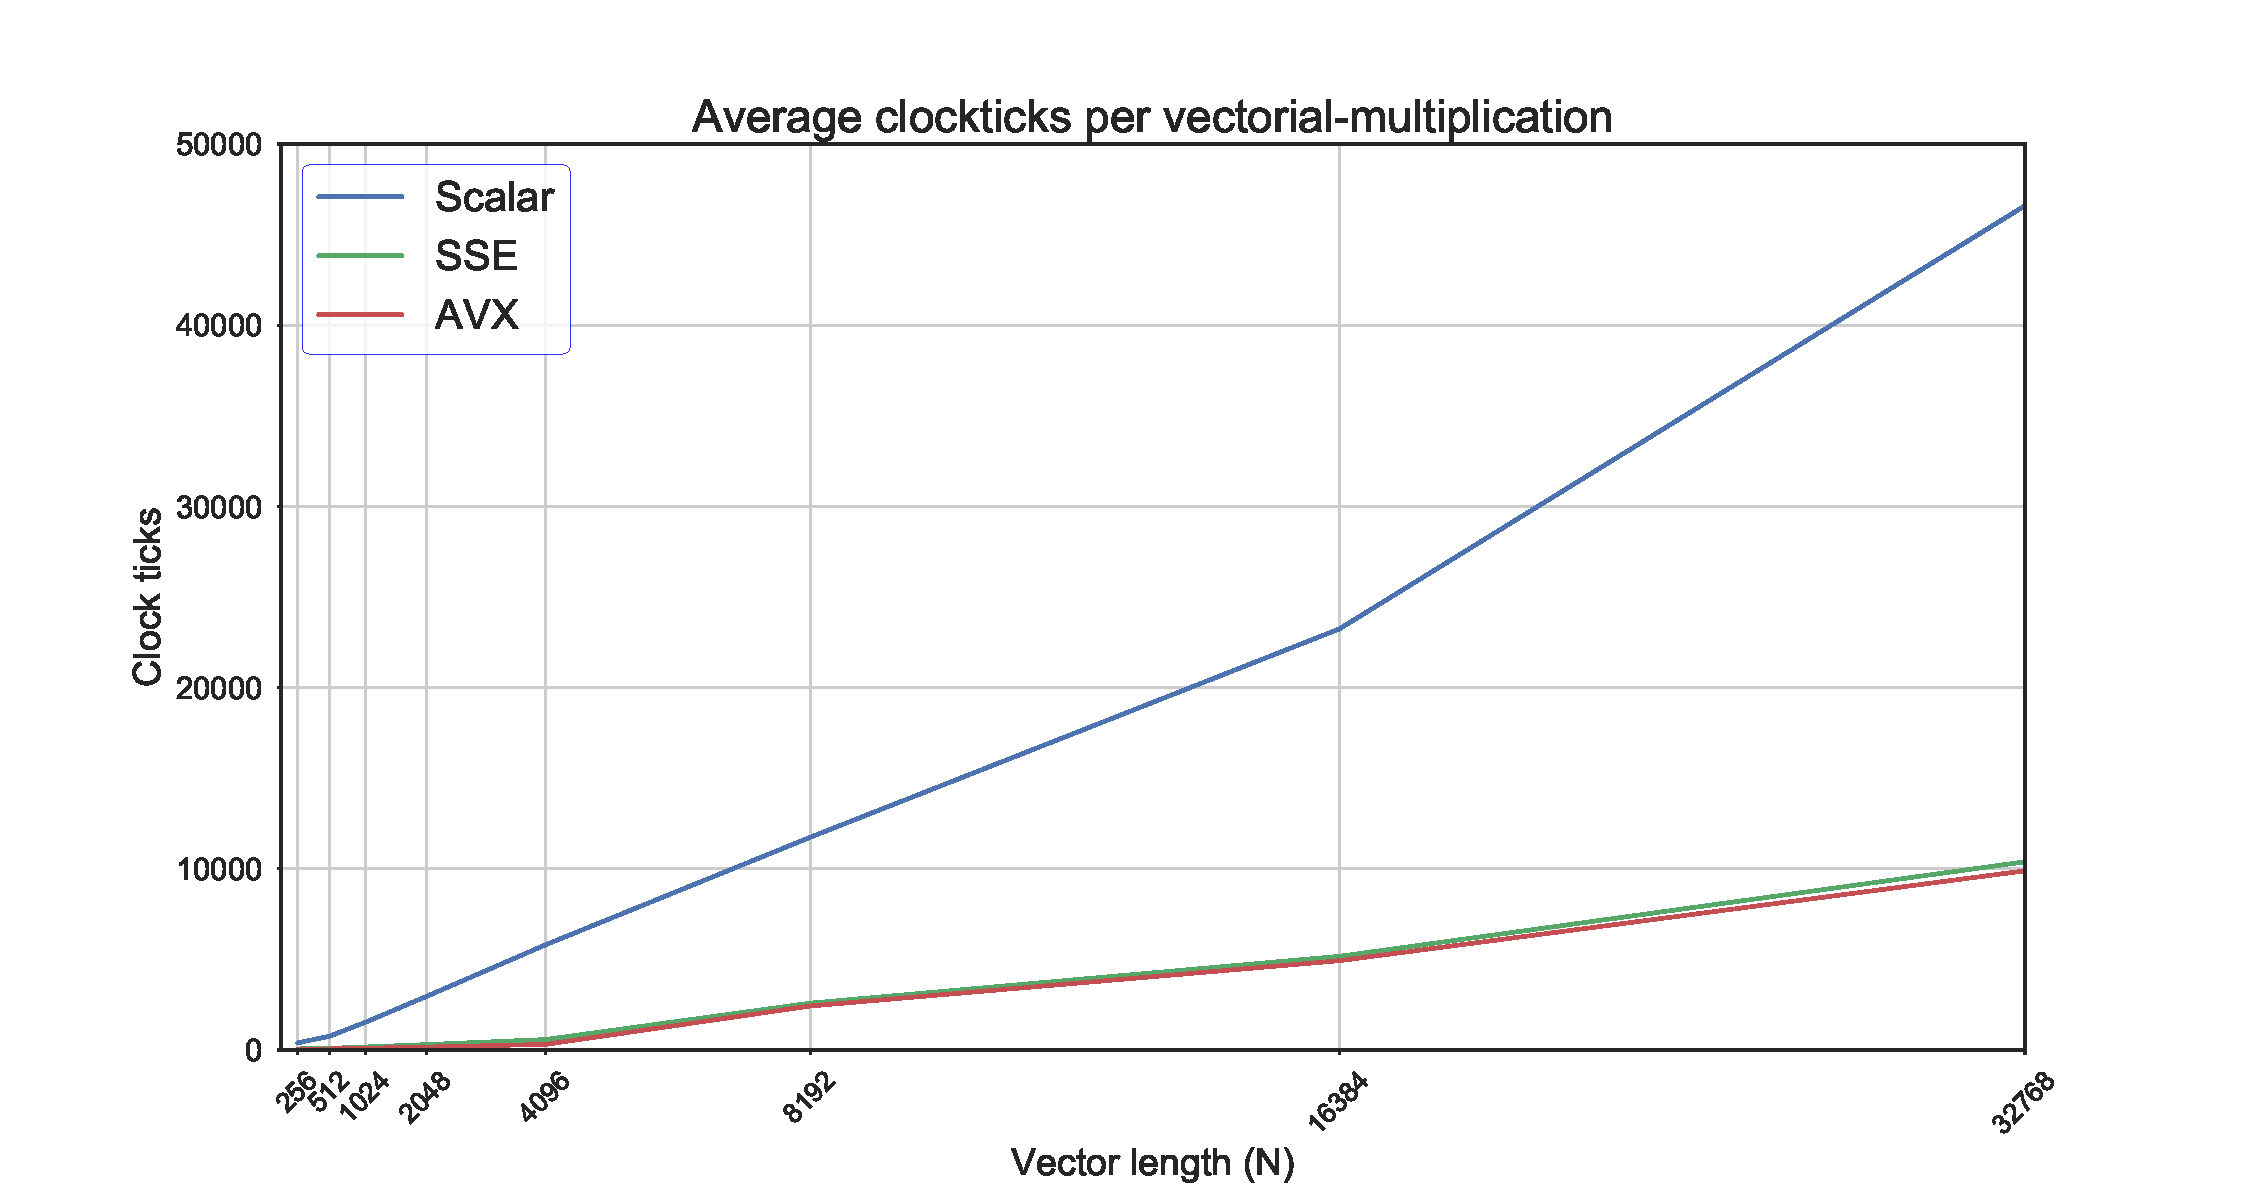
\includegraphics[width=\textwidth]{avg_O2.pdf}
\end{figure}

As we can see, as expected the average clock ticks needed to complete a vectorial multiplication
increases linearly with the number of points and we can immediately appreciate the
speedup that the SIMD introduces. To better evaluate the performance, let plot the
speedup with respect to the scalar baseline.\\

\begin{figure}[!ht]
    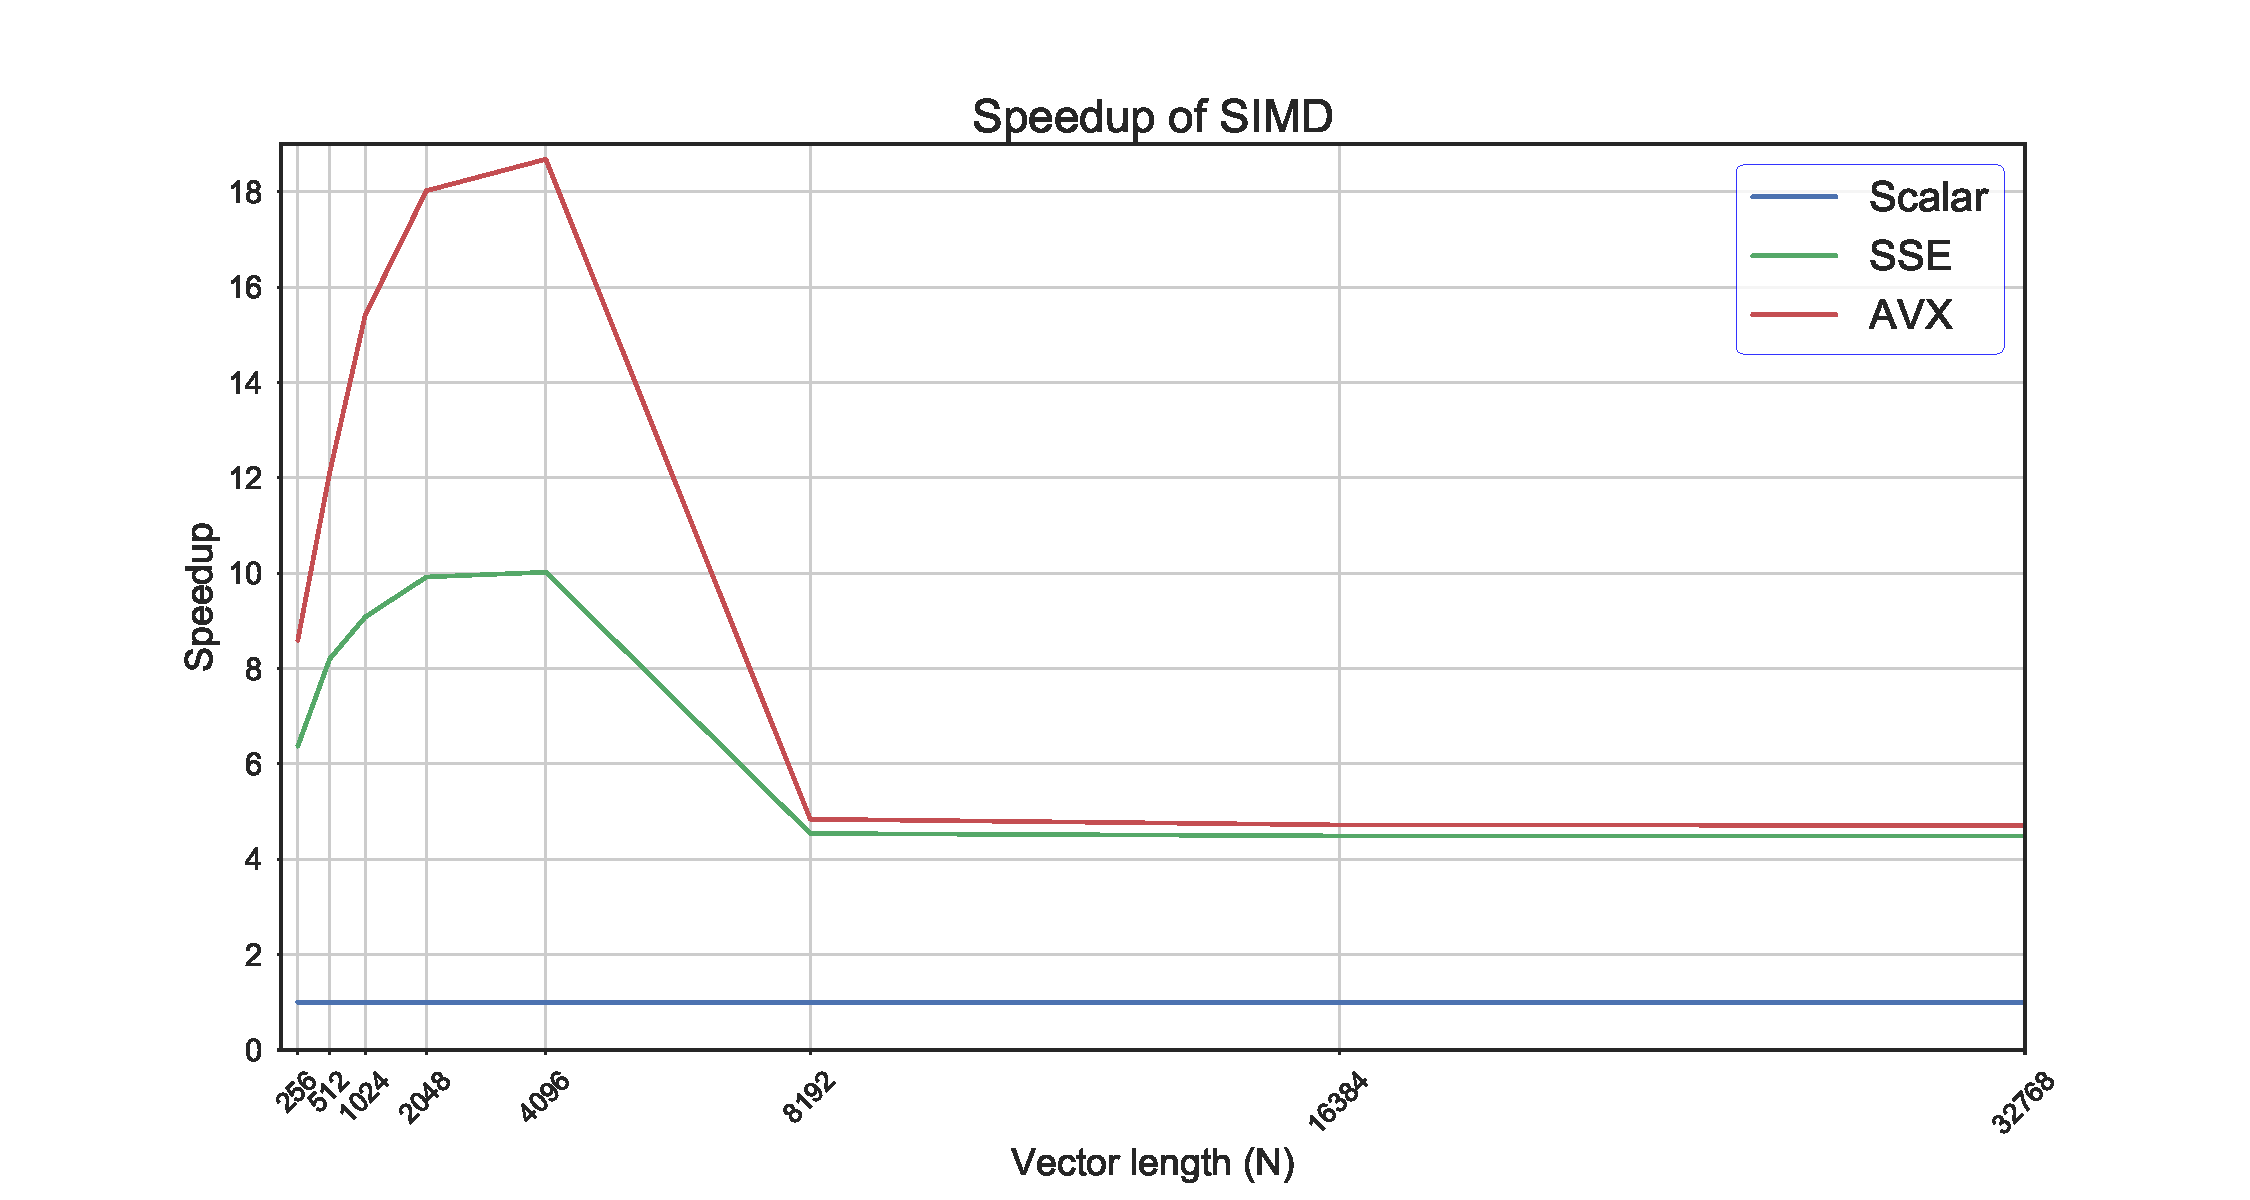
\includegraphics[width=\textwidth]{speedup_O2.pdf}
\end{figure}

Let's take for instance the case of N equal to 2048. The SSE introduces a 128 bits
parallelism and therefore eight 16-bits results can be computed can be computed at the
same time. We should have expected a plain 8X speedup, but the \texttt{-O2} optimization
was able to reduce the latency by a factor of 10. Similar for AVX, we expected a 16X
speedup with respect to the scalar baseline but instead the compiler produced a binary
upto 19 times faster than before. \\

Performances, though, seems to drastrically reduce for N equal to to 8192 and here
we might start having some caches problems: the set of operands arrays and the result
array ends up with 384KB of allocated memory which exceeds the available 256KB of L2 cache.
Unfortunatly, I did not find specifications of latency for the L3 cache and therefore
I cannot make comparisons on that.\\

Compiling the binary with the \texttt{-O3} flag, ended up with some interesting results.
\\
\begin{figure}[!ht]
    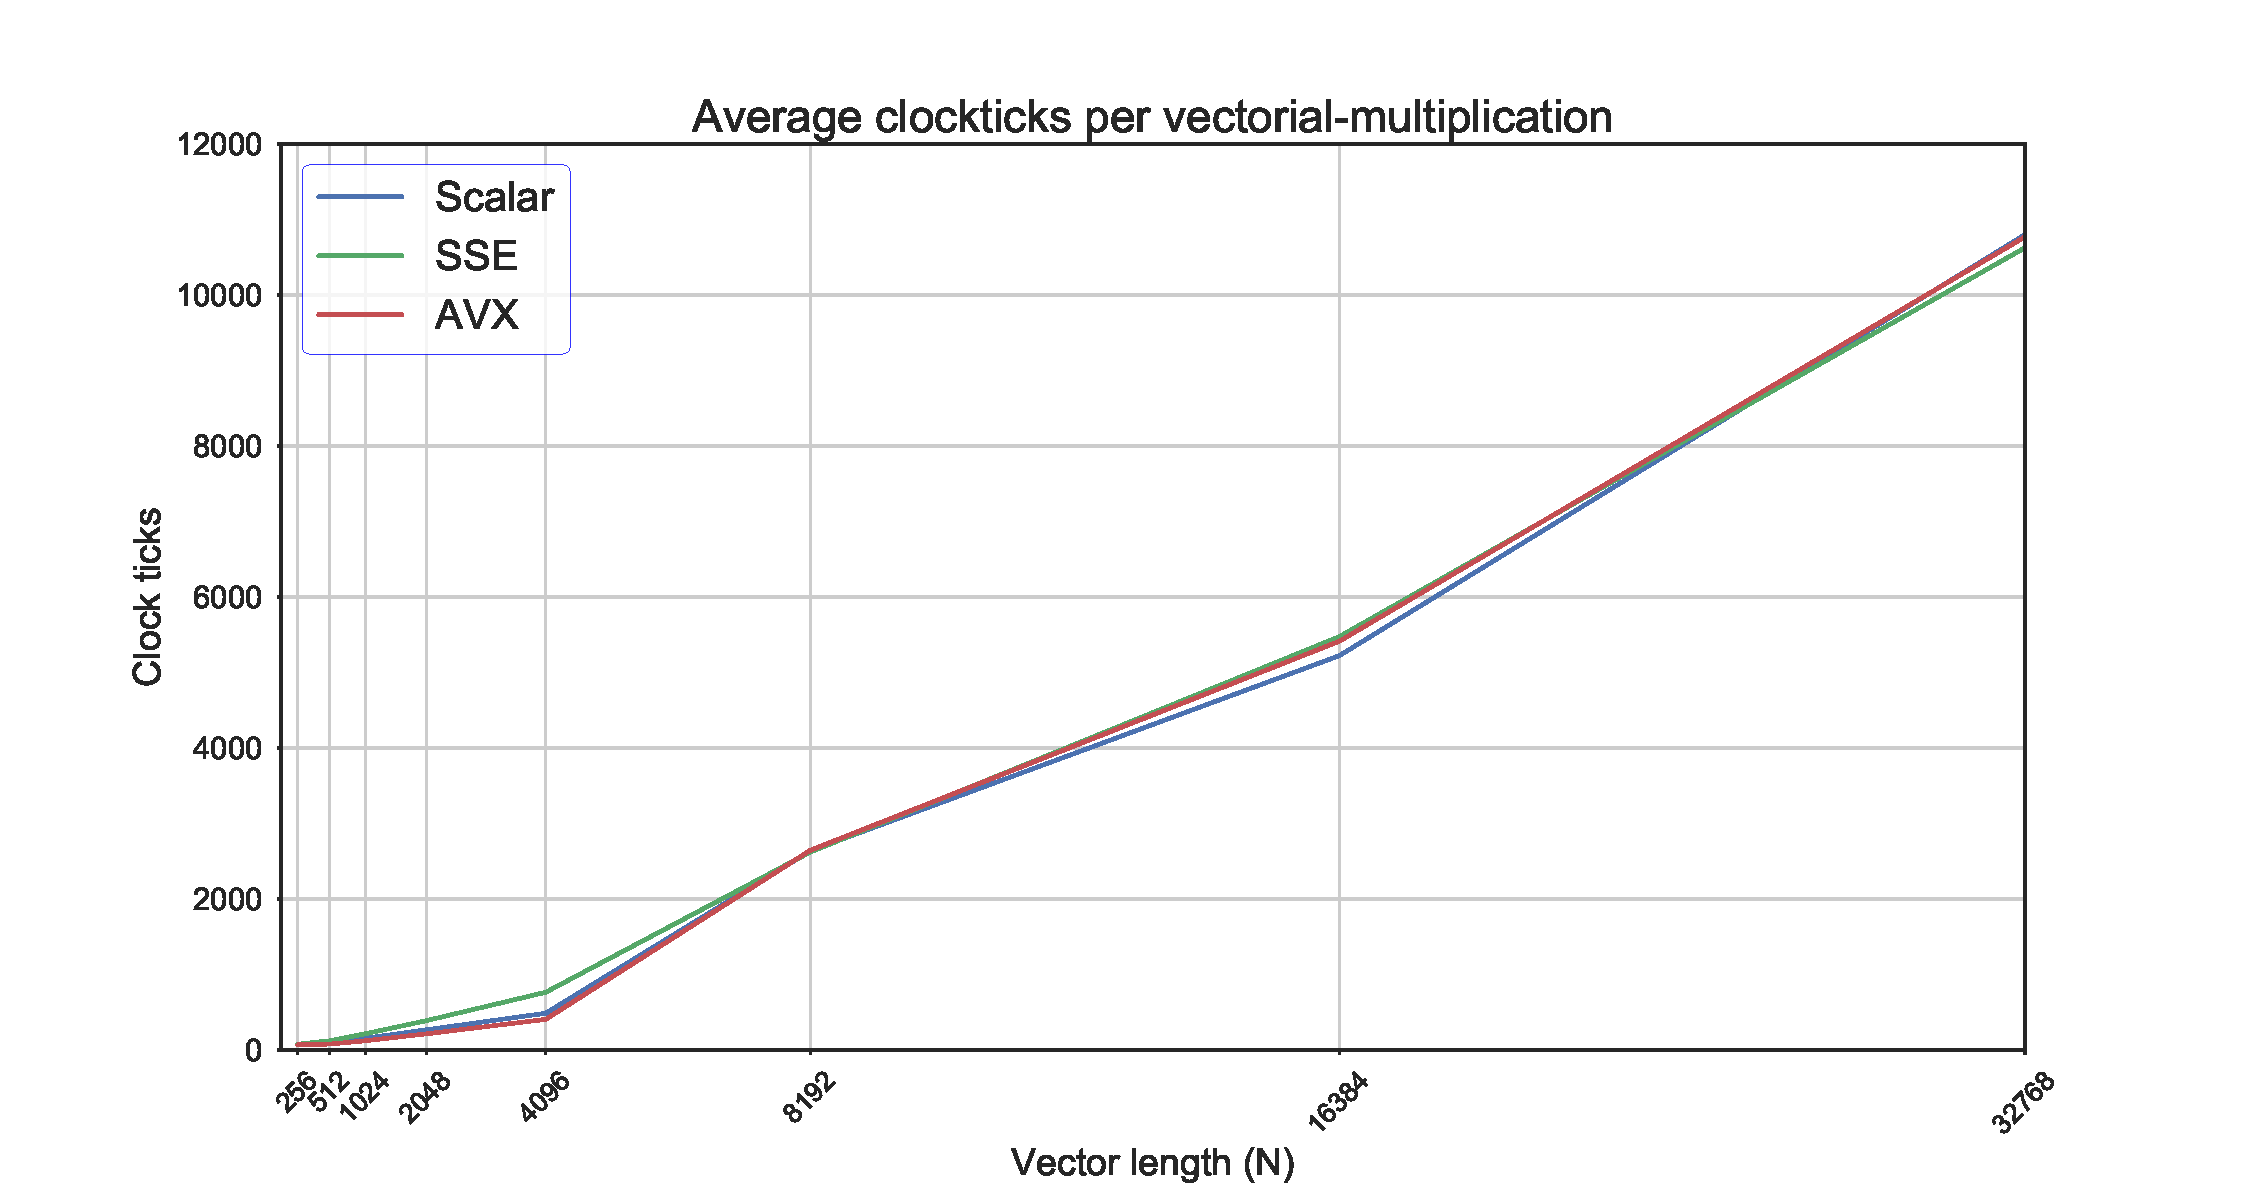
\includegraphics[width=\textwidth]{avg_O3.pdf}
    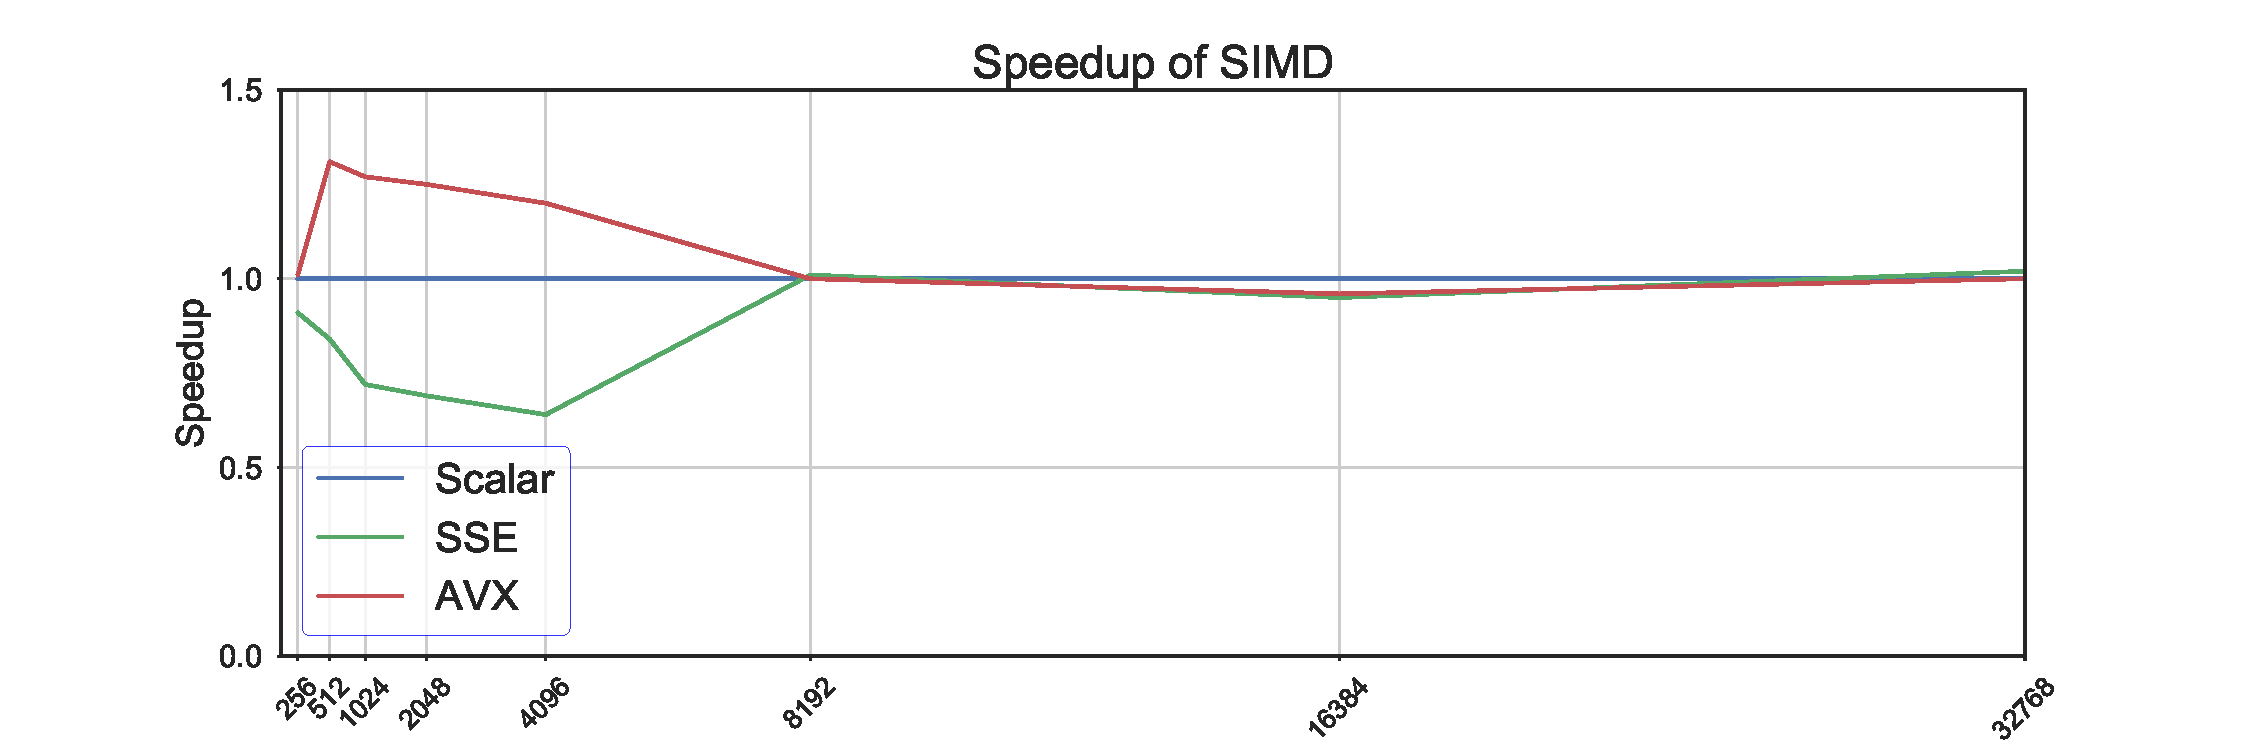
\includegraphics[width=\textwidth]{speedup_O3.pdf}
\end{figure}

The compiler was smart enough to understand that the operation we intended to do
could have been drastically speeded up using SIMD. Moreover, it's interesting to notice
that it automatically used the best version of the available SIMD: in fact, forcing
it to use SSE reduces the speedup. The same aforementioned caches issues can be found
also here starting at 8192 entries.

\end{document}
